\documentclass[a4paper,12pt]{article}
\usepackage[utf8]{inputenc}
\usepackage{polski}
\usepackage{float}
\usepackage{graphicx}
\usepackage{amsmath}
\usepackage{geometry}
\usepackage{hyperref}
\usepackage{listings}

\geometry{margin=2cm}

\begin{document} 

% Strona tytułowa
\begin{titlepage}
    \centering
    
	\begin{figure}[ht!]
	\centering
	
\includegraphics[width=170mm]{wmifs_pl.png}
	\vspace{0.5cm}
	\end{figure}    
    
    {\Huge \textbf{Sprawozdanie z projektu programistycznego}}\\[1cm]
    \rule{0cm}{0.5cm} % przerwa miedzy tekstem a zdjeciem
    
    {\LARGE Ciągi liczbowe z podciągami malejącymi}\\[1cm]
    
    \vspace{1cm}
    \large \textbf{Imię i Nazwisko} Daniel Olejasz \\
    \textbf{Numer grupy:} P05\\
    \textbf{Data:} 15 grudnia 2024\\
    
    \vfill
    {\large Środowisko: Code::Blocks IDE, język C++}\\
    \vspace{0.5cm}
    {\large GitHub jako repozytorium kodu}\\
    
    \vfill
\end{titlepage}

% Spis treści
\newpage
\tableofcontents
\newpage

% Wstęp - Treść zadania
\section{Treść zadania}
Dla zadanego ciągu liczbowego liczb całkowitych (w postaci tablicy) znajdź liczbę wszystkich podciągów malejących (Podciąg musi składać się z przynajmniej dwóch wartości). \\ \\
Przykład:
\begin{flushleft}
\textbf{Wejście:} A[] = [5, 4, 2, 2, 1] \\
\textbf{Wyjście:} Liczba wszystkich podciągów malejących to 4 \\
\text{[5, 4], [5, 4, 2], [4, 2], [2, 1]}
\end{flushleft}

\begin{flushleft}
\textbf{Wejście:} A[] = [2, 5, 3] \\
\textbf{Wyjście:} Liczba wszystkich podciągów malejących to 1 \\
\text{[5, 3]}
\end{flushleft}

\begin{flushleft}
\textbf{Wejście:} A[] = [5, 4, 2, 2, 1] \\
\textbf{Wyjście:} Liczba wszystkich podciągów malejących to 0
\end{flushleft}


\section{Rozwiązywanie problemu}
\subsection{Podejście pierwsze - stałe tablice}

\subsubsection{Opis problemu}

Program rozwiązuje problem znajdowania wszystkich malejących podciągów w zadanych tablicach liczb całkowitych oraz ich liczby. Każdy podciąg musi składać się z co najmniej dwóch liczb i musi spełniać warunek, że każdy kolejny element jest mniejszy od poprzedniego. Dane wejściowe są pobierane z pliku tekstowego, a wyniki (lista malejących podciągów i ich liczba) są zapisywane do innego pliku tekstowego.

\subsubsection{Struktura danych wejściowych i wyjściowych}

Wejście (plik \texttt{input.txt}):

\begin{flushleft}
\begin{enumerate}
	\item{Liczba tablic (\texttt{numArrays})}
	\item{Dla każdej tablicy: }
	\begin{itemize}
		\item{Liczba elementów tablicy (\texttt{n})}
		\item{\texttt{n} liczb całkowitych, stanowiących elementy tablicy}
	\end{itemize}
\end{enumerate}
\end{flushleft}

\begin{flushleft}
Wyjście (plik \texttt{output.txt}):
\begin{enumerate}
	\item{Lista wszystkich malejących podciągów dla każdej tablicy}
	\item{Łączna liczba tych podciągów}
\end{enumerate}
\end{flushleft}

\newpage

\subsubsection{Opis działania programu}

\begin{enumerate}
\item{Wczytywanie danych z pliku}
\begin{itemize}
\item{Program otwiera plik wejściowy \texttt{input.txt}. Jeśli plik nie istnieje lub wystąpi problem z jego otwarciem, program zgłasza błąd i kończy działanie.}
\item{Z pierwszej linii pliku wczytywana jest liczba tablic (\texttt{numArrays})}
\item{Następnie dla każdej tablicy:}
\begin{itemize}
\item[\textbullet]{Wczytywany jest jej rozmiar (\texttt{n})}
\item[\textbullet]{Wczytywane jest \texttt{n} elementów tablicy do lokalnej tablicy \texttt{arr}}
\end{itemize}
\end{itemize}
\item{Przetwarzanie danych}\\ \\
Dla każdej tablicy program:
\begin{itemize}
\item{Wypisuje jej zawartość do pliku wyjściowego \texttt{output.txt}.}
\item{Przetwarza tablice, szukając wszystkich malejących podciągów za pomocą funkcji \texttt{Subarrays}.}
\end{itemize}
\item{Funkcja \texttt{Subarrays}}
\begin{itemize}
\item{Funkcja przyjmuje:}
\begin{itemize}
\item[\textbullet]{Tablicę liczb całkowitych \texttt{arr}.}
\item[\textbullet]{Liczbę elementów tablicy \texttt{n}.}
\item[\textbullet]{Referencję do obiektu pliku wyjściowego \texttt{outputFile}}
\end{itemize}
\end{itemize}
\item{Działanie funkcji}
\begin{itemize}
\item{Sprawdza, czy długość tablicy jest mniejsza niż 2. Jeśli tak, wypisuje komunikat, że nie ma możliwych malejących podciągów.}
\item{Zlicza liczbę malejących podciągów:}
\begin{itemize}
\item[\textbullet]{Utrzymuje indeks \texttt{start} jako początek aktualnej malejącej sekwencji.}
\item[\textbullet]{Iteruje po tablicy sprawdzając warunek \texttt{arr[i]<arr[i-1]}.}
\item[\textbullet]{Gdy napotka element, który nie spełnia tego warunku, wypisuje wszystkie możliwe podciągi wynikające z bieżącej sekwencji do pliku wyjściowego.}
\item[\textbullet]{Po zakończeniu iteracji przetwarza ostatnią sekwencję, jeśli zakończyła się na końcu tablicy.}
\end{itemize}
\item{Zapisuje liczbę znalezionych podciągów do pliku.}
\end{itemize}
\item{Zapisywanie wyników do pliku}
\begin{itemize}
\item{Wszystkie malejące podciągi są zapisywane do pliku wyjściowego, każdy w formacie \texttt{[a,b,c,...]}.}
\item{Po każdym zestawie podciągów dla tablicy program dodaje liczbę znalezionych podciągów.}
\end{itemize}
\item{Zamknięcie plików}
\begin{itemize}
\item{Program zamyka pliki wejściowy i wyjściowy po zakończeniu działania.}
\end{itemize}
\end{enumerate}

\newpage

\subsubsection{Schemat blokowy algorytmu}
W tym miejscu znajduję się schemat blokowy dla funkcji \texttt{Subarrays}. Ilustruje on zasadę jej działania:

\begin{figure}[H]
    \centering
    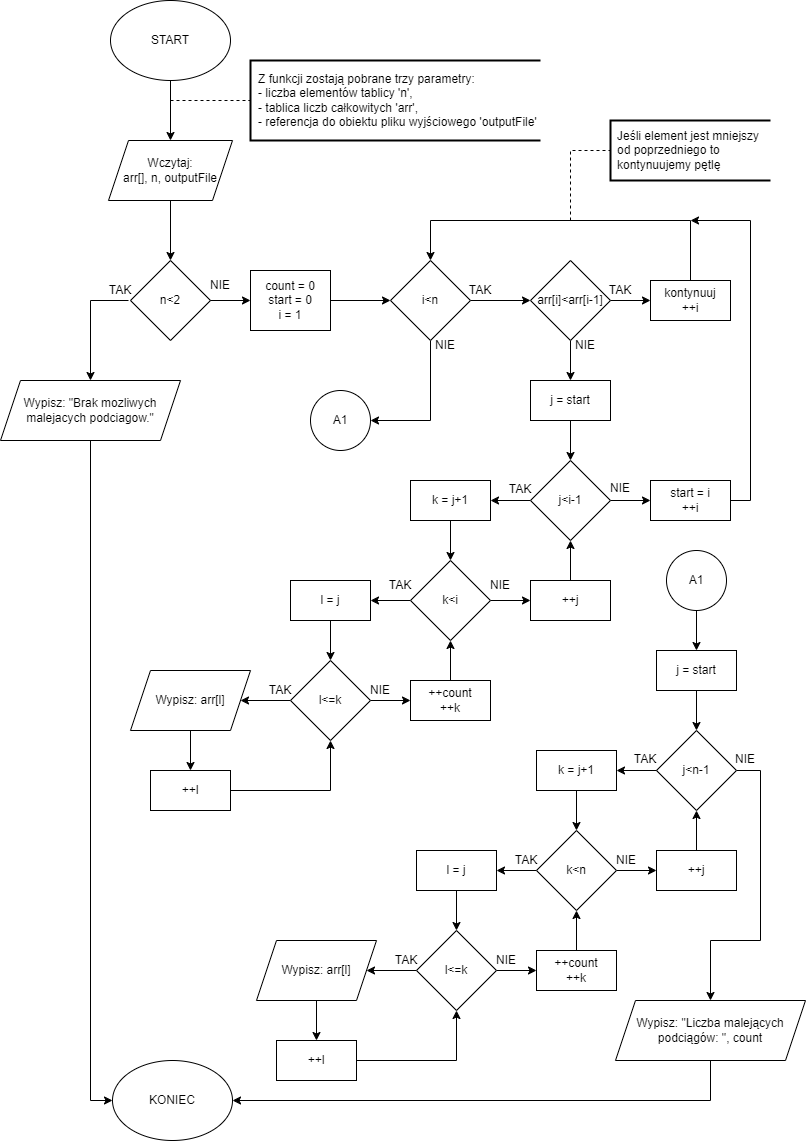
\includegraphics[width=0.9\textwidth]{Schemat1r.png}
    \caption{Schemat blokowy funkcji \texttt{Subarrays}.}
    \label{fig:schemat_Subarrays1}
\end{figure}

\newpage

\subsubsection{Pseudokod algorytmu}

\underline{Pseudokod dla funkcji \texttt{Subarrays} rozwiązującej zadany problem: } 
\begin{verbatim}
Funkcja Subarrays(arr, n, outputFile):
    Jeśli n < 2:
        Wypisz "Brak mozliwych malejacych podciagow" do pliku
        Zakończ funkcję
    Zainicjalizuj zmienną "count" na 0
    Zainicjalizuj zmienną "start" na 0
    Dla i od 1 do n-1:
        Jeśli arr[i] < arr[i-1]:
            Kontynuuj pętlę
        Inaczej:
            Dla j od start do i-2:
                Dla k od j+1 do i-1:
                    Wypisz podciąg [arr[j], arr[j+1], ..., arr[k]] do pliku
                    Zwiększ count o 1
            Ustaw start na i
    Dla j od start do n-2:
        Dla k od j+1 do n-1:
            Wypisz podciąg [arr[j], arr[j+1], ..., arr[k]] do pliku
            Zwiększ count o 1
    Wypisz "Liczba malejacych podciagow: count" do pliku
\end{verbatim}

\newpage

\subsection{Drugie podejście - dynamiczne tablice}
\subsubsection{Opis problemu - pytanie o usprawnienie programu}
W tym miejscu warto zadać sobie pytanie, czy jest możliwe napisanie kodu programu, który będzie zawierał mniej pętli \texttt{for}, a co za tym idzie będzie skutkował niższą złożonością obliczeniową? Odpowiedź brzmi: \textbf{Tak, ale nie do końca.}

Obniżenie złożoności czasowej programu wymaga optymalizacji działania funkcji \texttt{Subarrays}, ponieważ jest to główny element wpływający na czas wykonania programu. Funkcja ta generuje wszystkie malejące podciągi w sposób nieefektywny, przeszukując wszystkie możliwe kombinacje, co powoduje złożoność \texttt{O(n\textsuperscript{3})} (więcej o złożoności obliczeniowej w kolejnym rozdziale).

W jaki więc sposób można częściowo rozwiązać to zadanie tak, aby złożoność obliczeniowa była mniejsza? Poniżej przedstawiam sposób na rozwiązanie tego problemu opisując samą funkcję:

\subsubsection{Opis działania omawianej funkcji}

\begin{enumerate}
\item{Wczytywanie danych}
\begin{itemize}
\item{Funkcja otrzymuję tablicę \texttt{arr} oraz liczbę jej elementów \texttt{n}.}
\item{Wewnątrz funkcji tworzone są zmienne \texttt{licznik = 0} oraz \texttt{dlugosc = 1}.}
\end{itemize}
\item{Przetwarzanie danych}\\ \\
Dla każdej tablicy funkcja (CountDecreasingSubarrays):
\begin{itemize}
\item{Sprawdza, czy długość tablicy jest mniejsza od 2. Jeśli tak, to zwraca liczbę 0 (ponieważ nie znajdują się tam żadne podciągi malejące).}
\item{Wypisuje liczbę podciągów.}
\end{itemize}
\item{Funkcja \texttt{CountDecreasingSubarrays}}
\begin{itemize}
\item{Funkcja przyjmuje:}
\begin{itemize}
\item[\textbullet]{Tablicę liczb całkowitych \texttt{arr}.}
\item[\textbullet]{Liczbę elementów tablicy \texttt{n}.}
\end{itemize}
\item{Następnie funkcja iteruję przez tablicę (porównuje kolejne elementy tablicy):}
\begin{itemize}
\item[\textbullet]{Jeśli element jest mniejszy od poprzedniego, wydłużamy bieżącą sekwencję malejącą \texttt{(dlugosc)}.}
\item[\textbullet]{Jeśli nie jest, obliczamy liczbę podciągów dla zakończonego fragmentu malejącego i resetujemy długość.}
\item[\textbullet]{Po zakończeniu pętli dodajemy podciągi dla ostatniego fragmentu malejącego.}
\end{itemize}
\end{itemize}
\item{Wyświetlanie wyników}
\begin{itemize}
\item{Na koniec funkcja zwraca łączną liczbę malejących podciągów.}
\end{itemize}
\end{enumerate}


Zatem częściowym rozwiązaniem programu byłaby taka funkcja, która \textbf{tylko} zlicza ilość malejących podciągów, bez ich wypisania. Zmniejsza to czytelność wyników, gdyż nie otrzymujemy wypisanych podciągów tylko ich liczbę, ale skorzystanie z takiej funkcji ma też swoje zalety. Ta funkcja ma złożoność obliczeniową \texttt{O(n)}, co jest bardzo dużą różnicą względem poprzedniej funkcji.

Zatem w przypadku implementacji takiej funkcji w innym programie warto się zastanowić nad jej użyciem zamiast funkcji \texttt{Subarrays}, w przypadku gdy nie potrzebujemy znać podciągów, lecz tylko ich liczbę.

\newpage

\subsubsection{Schemat blokowy funkcji CountDecreasingSubarrays}
W tym miejscu znajduję się schemat blokowy omawianej funkcji \texttt{CountDecreasingSubarrays}. Przedstawia on zasadę jej działania:

\begin{figure}[H]
    \centering
    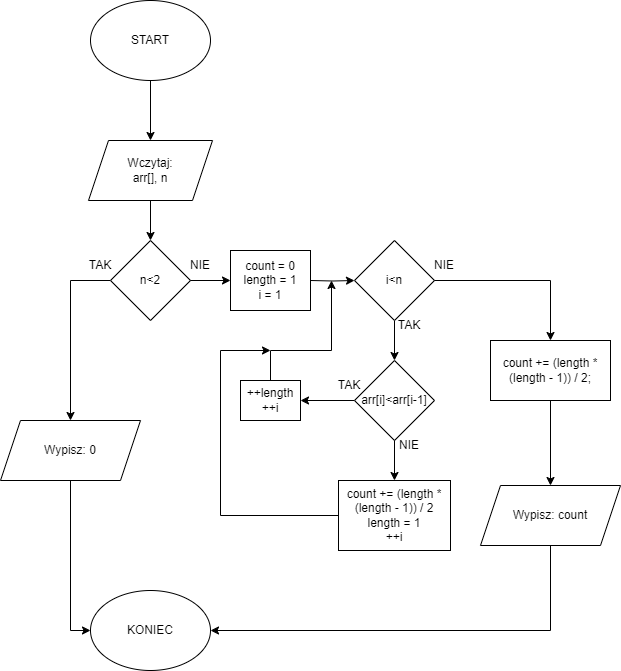
\includegraphics[width=0.9\textwidth]{Schemat2r.png}
    \caption{Schemat blokowy funkcji \texttt{CountDecreasingSubarrays}.}
    \label{fig:schemat_CountDecreasingSubarrays1}
\end{figure}

\newpage

\subsubsection{Pseudokod funkcji CountDecreasingSubarrays}

\underline{Pseudokod dla funkcji \texttt{CountDecreasingSubarrays} rozwiązującej zadany problem: } 
\begin{verbatim}
Funkcja CountDecreasingSubarrays(arr, n):
    Jeśli n < 2:
        Wypisz 0 
        Zakończ funkcję
    Zainicjalizuj zmienną "count" na 0
    Zainicjalizuj zmienną "length" na 1
    Dla i od 1 do n-1:
        Jeśli arr[i] < arr[i-1]:
            Zwiększ length o 1
        Inaczej:
            Wykonaj count += (length * (length - 1)) / 2;
            Ustaw length na 1
    Wykonaj count += (length * (length - 1)) / 2;
    Wypisz "Liczba malejacych podciagow: count"
\end{verbatim}

\newpage

\subsection{Implementacja obu podanych funkcji}

\subsubsection{Pierwsza wersja}

Zaimplementujemy teraz nasze pierwsze opisane podejście. Mamy już schemat tego jak funkcja powinna wyglądać oraz jej zarys w pseudokodzie, zatem zostaję ją teraz zapisać w języku \texttt{C++}.

\begin{figure}[H]
    \centering
    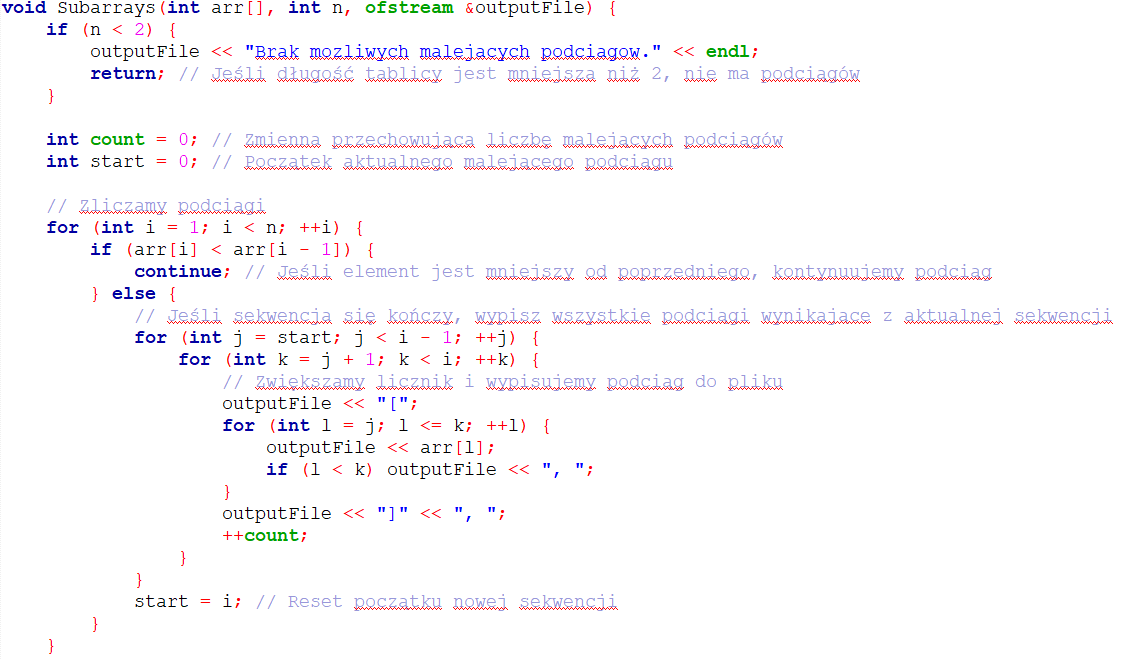
\includegraphics[width=0.9\textwidth]{Implement1.png}
    \caption{Implementacja pierwszej metody.}
    \label{fig:schemat_Implement1}
\end{figure}

\begin{figure}[H]
    \centering
    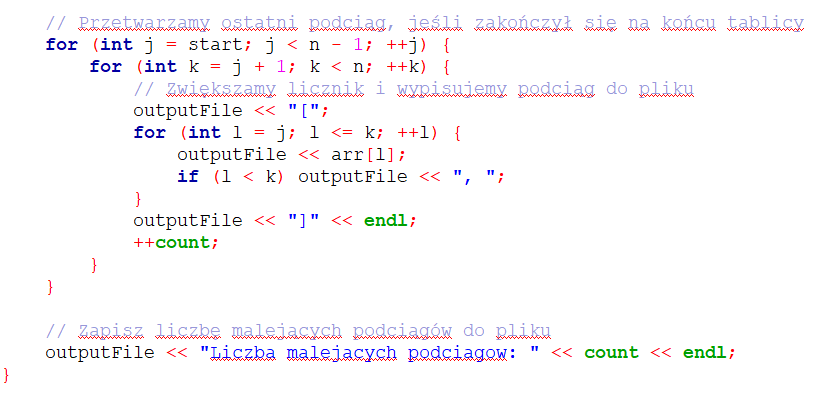
\includegraphics[width=0.9\textwidth]{Implement2.png}
    \caption{Implementacja pierwszej metody.}
    \label{fig:schemat_Implement2}
    \rule{0cm}{1.3cm} % przerwa miedzy tekstem a zdjeciem
    Funkcja \texttt{Subarrays} po utworzeniu w języku \texttt{C++} wygląda następująco.
\end{figure}

\newpage

Tworzymy teraz nasz plik wejściowy i dodajemy do niego dane. Zgodnie z oczekiwanym przez program wejściem, plik \texttt{input.txt} będzie wyglądał następująco: 

\begin{verbatim}
4
5 5 4 2 2 1
3 2 5 3
5 1 2 4 6 7
4 8 6 4 2
\end{verbatim}

Następnie w głównej funkcji \texttt{main} programu wywołujemy naszą utworzoną funkcję \texttt{Subarrays}.

\begin{figure}[H]
    \centering
    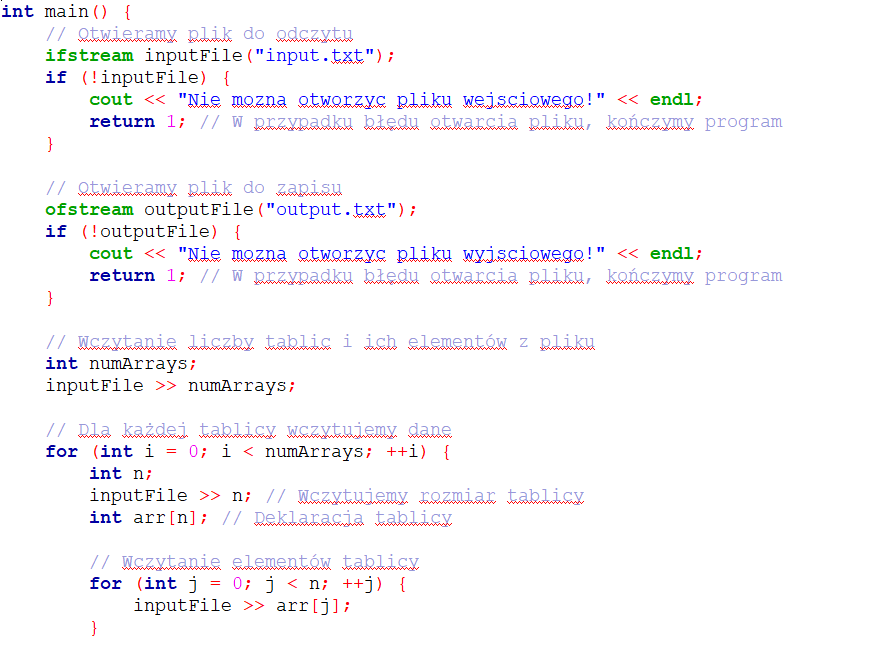
\includegraphics[width=0.8\textwidth]{Implement3.png}
    \caption{Wywoływanie pierwszej metody.}
    \label{fig:schemat_Implement3}
\end{figure}

\begin{figure}[H]
    \centering
    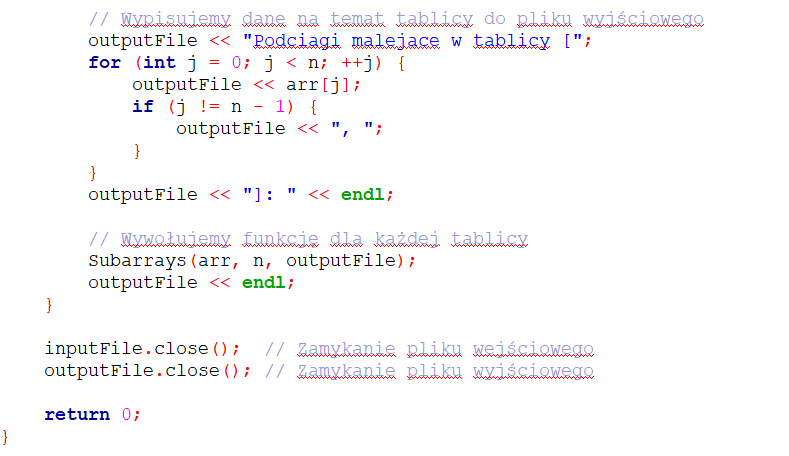
\includegraphics[width=0.8\textwidth]{Implement4.png}
    \caption{Wywoływanie pierwszej metody.}
    \label{fig:schemat_Implement4}
\end{figure}

\newpage

\subsubsection{Druga wersja}

Zaimplementujemy teraz nasze drugie opisane podejście. Tutaj także mamy już schemat tego jak funkcja powinna wyglądać oraz jej zarys w pseudokodzie, zatem zapisujemy ją teraz w języku \texttt{C++}. Posłużę się tutaj dodatkową funkcją \texttt{RunTests}, która odpowiedzialna jest za testy poprawności naszych funkcji.

\begin{figure}[H]
    \centering
    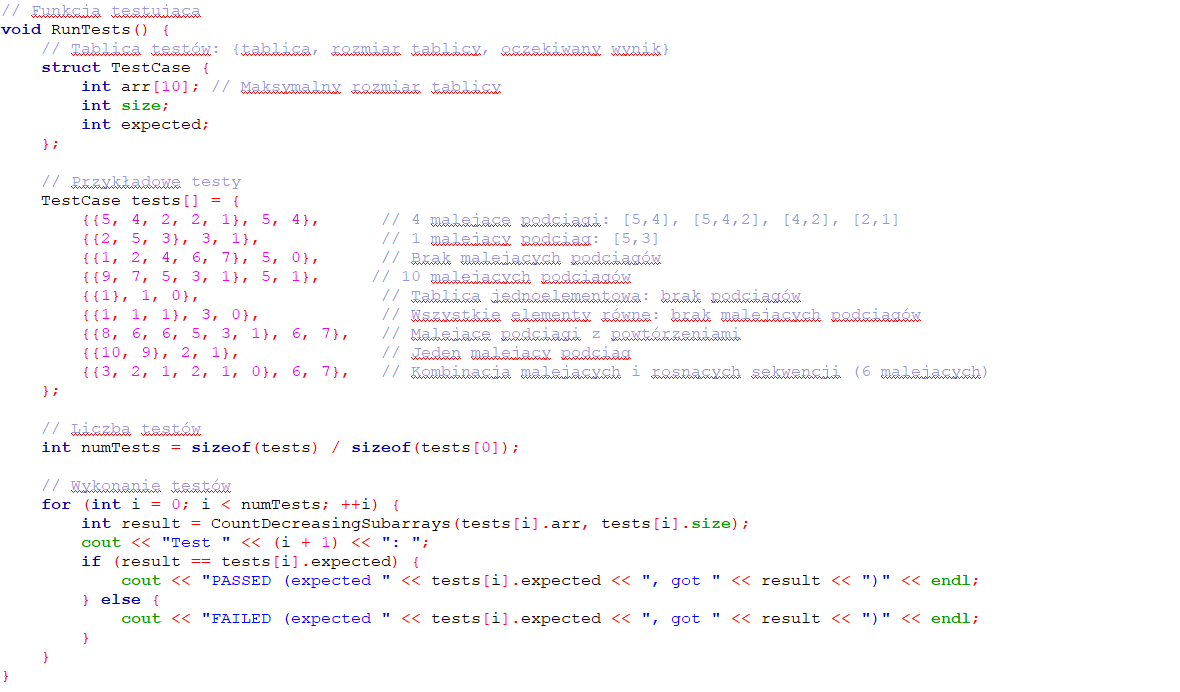
\includegraphics[width=1\textwidth]{RunTests1.png}
    \caption{Funkcja pomocnicza \texttt{RunTests} sprawdzająca poprawność działania programu.}
    \label{fig:RunTests1}
\end{figure}

\begin{figure}[H]
    \centering
    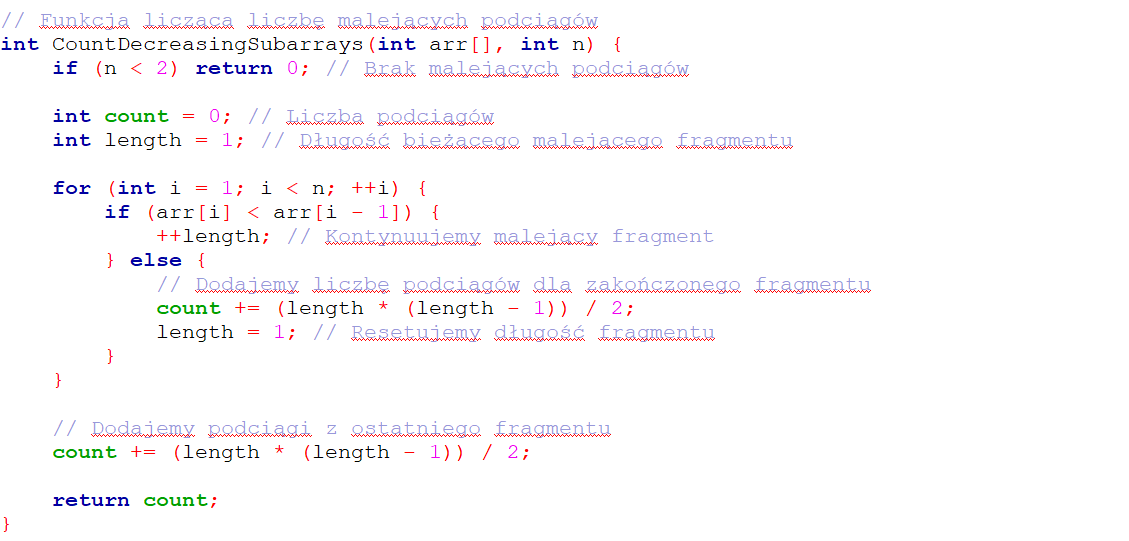
\includegraphics[width=1\textwidth]{Count1.png}
    \caption{Funkcja \texttt{CountDecreasingSubarrays} zliczająca ilość podciągów malejących.}
    \label{fig:Count1}
\end{figure}

\newpage

Funkcja \texttt{main} zawierająca wywołanie wszystkich innych funkcji prezentuje się następująco:

\begin{figure}[H]
    \centering
    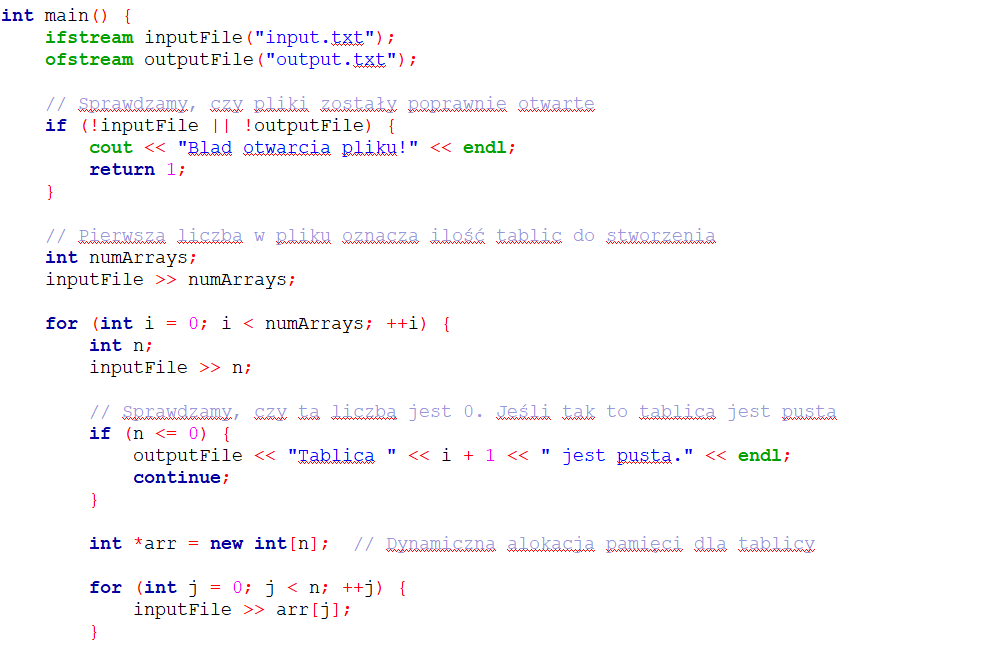
\includegraphics[width=1\textwidth]{Implement5.png}
    \caption{Wywołanie funkcji w \texttt{main}.}
    \label{fig:Implement5}
\end{figure}

\begin{figure}[H]
    \centering
    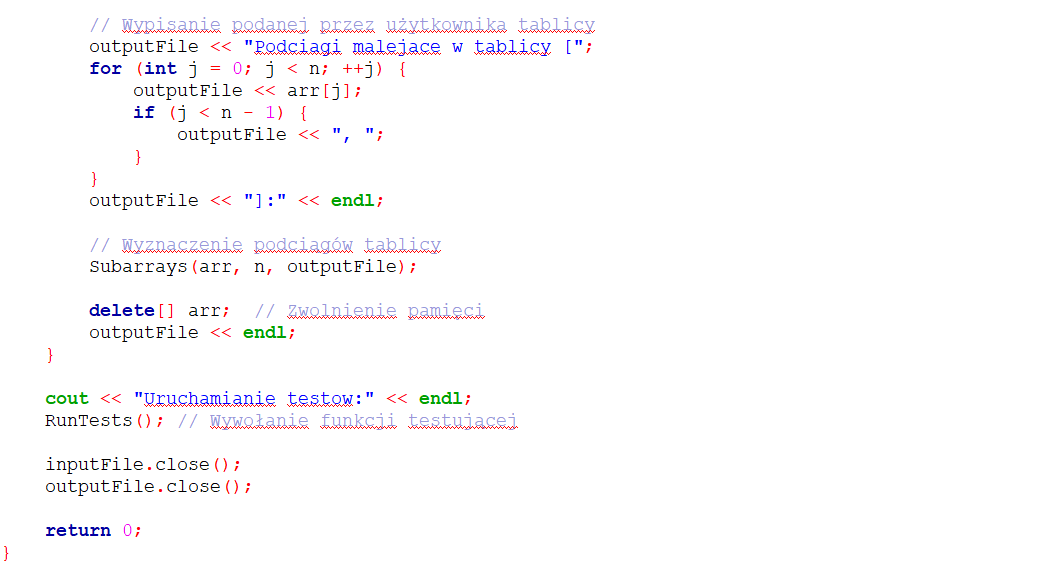
\includegraphics[width=1\textwidth]{Implement6.png}
    \caption{Wypisanie podciągów przed wyliczeniem i wyznaczeniem podciągów malejących.}
    \label{fig:Implement6}
\end{figure}

\newpage

\section{Podstawy teoretyczne}
\subsection{Złożoność czasowa, pamięciowa i obliczeniowa}
Przejdźmy teraz do złożoności obliczeniowej. Złożoność ta określa jak wielką ilość zasobów potrzeba do rozwiązania problemu obliczeniowego. Rozważmy teraz te kwestię dla obu wersji programu.

\subsubsection{Złożoności dla pierwszej wersji programu}

\begin{enumerate}
\item{Złożoność czasowa}:

Główna część obliczeń znajduje się w funkcji \texttt{Subarrays}. Przeanalizujmy ją szczegółowo:
\begin{itemize}
\item{Pętla zewnętrzna ze zmienną \texttt{i} iteruje przez elementy tablicy, czyli O(n).}
\item{Wewnętrzne przetwarzanie podciągów (gdy kończy się sekwencja malejąca):}
\begin{itemize}
\item{Pierwsza pętla: \texttt{j} iteruje od \texttt{start} do \texttt{i-1}, czyli w najgorszym przypadku O(n).}
\item{Druga pętla: \texttt{k} iteruje od \texttt{j+1} do \texttt{i}, co daje \texttt{O(n-j)} iteracji, ale w najgorszym przypadku również O(n).}
\item{Trzecia pętla: \texttt{l} iteruje od \texttt{j} do \texttt{k}, czyli O(n) w najgorszym przypadku.}
\end{itemize}
\end{itemize}
Łączna liczba iteracji w najgorszym przypadku dla wszystkich trzech pętli to O(n\textsuperscript{3}).

\textbf{Ostatni podciąg (po zakończeniu głównej pętli):} Podobnie jak poprzedni fragment, jego złożoność w najgorszym przypadku wynosi O(n\textsuperscript{3}).

Podsumowując:

Dla każdej tablicy, złożoność funkcji \texttt{Subarrays} wynosi O(n\textsuperscript{3}). Zakładając, że mamy \texttt{m} tablic, każda o maksymalnym rozmiarze \texttt{n}, złożoność wynosi: O(m*n\textsuperscript{3}).

\item{Złożoność pamięciowa}

Główne aspekty pamięci programu:
\begin{itemize}
\item{Tablica wejściowa \texttt{arr}: Dla każdej tablicy deklarowanej dynamicznie w pętli \texttt{n} elementów, potrzebujemy O(n) pamięci.}
\item{Alokacja w funkcji \texttt{Subarrays}: Żadne dodatkowe struktury nie są tworzone poza zmiennymi lokalnymi \texttt{start}, \texttt{count}, itp., więc zużycie pamięci dla funkcji jest O(1).}
\item{Łączne zużycie pamięci: Zużycie pamięci przez funkcję dla każdej tablicy to O(n) (dane wejściowe). Przy \texttt{m} tablicach, całkowite zużycie pamięci to: O(n+m).}
\end{itemize}
\item{Złożoność obliczeniowa}

Złożoność obliczeniowa jest zgodna z analizą czasową, ponieważ każda iteracja lub operacja przyczynia się do złożoności czasowej. Podstawowa operacja to sprawdzenie warunku i zapis do pliku. Podsumowanie: 
\begin{itemize}
\item{Główna złożoność: O(m*n\textsuperscript{3}).}
\item{Każda iteracja i zapis do pliku stanowi jednostkę obliczeniową.}
\end{itemize}
\end{enumerate}

\textbf{Wnioski:}
\begin{enumerate}
\item{Czasowa: O(m*n\textsuperscript{3}) – dominuje analiza podciągów.}
\item{Pamięciowa: O(n+m) – wynika z tablicy wejściowej i liczby tablic.}
\item{Obliczeniowa: O(m*n\textsuperscript{3}) – proporcjonalna do czasu.}
\end{enumerate}

\newpage

\subsubsection{Złożoności dla drugiej wersji programu}

Jako iż program korzysta z funkcji \texttt{Subarrays} jego złożoność obliczeniowa nie uległa zmianie. Natomiast gdyby zmienić program tak, aby wypisywał tylko i wyłącznie liczbę malejących podciągów, a co za tym idzie korzystał tylko z funkcji \texttt{CountDecreasingSubarrays}, to jego złożoność wyglądałaby następująco:

\begin{enumerate}
\item{Złożoność czasowa:}
Zamiast generować wszystkie malejące podciągi i wypisywać je osobno, możemy iterować po tablicy i zapisywać tylko informacje o liczbie podciągów malejących. Wystarczy przechodzić po tablicy i dla każdej sekwencji malejącej obliczyć liczbę podciągów za pomocą wzoru:

\texttt{$$Liczba\_podciagow= \frac{length\cdot(length-1)}{2}$$ }gdzie length to długość bieżącej sekwencji malejącej. Iterujemy przez tablicę raz, więc złożoność wynosi: O(n).
\item{Złożoność pamięciowa:}
Nie tworzymy żadnych dodatkowych struktur, poza zmiennymi licznikami, zatem złożoność pamięciowa wynosi: O(1).
\item{Złożoność obliczeniowa:}
Podobnie jak poprzednio, w tym przypadku złożoność obliczeniowa odpowiada złożoności czasowej, zatem wynosi ona: O(n)
\end{enumerate}

\textbf{Wnioski:}
\begin{enumerate}
\item{Czasowa: O(n) – jednorazowe przejście pętli.}
\item{Pamięciowa: O(1) – nie tworzymy żadnych dodatkowych zmiennych}
\item{Obliczeniowa: O(n) – proporcjonalna do czasu.}
\end{enumerate}

\rule{0cm}{0.5cm} % przerwa miedzy tekstem a zdjeciem

Jak widzimy sama funkcja \texttt{CountDecreasingSubarrays} ma znacznie mniejszą złożoność, a co za tym idzie, w przypadku pliku z większą ilością tablic skończy działanie szybciej (chociaż zrobi to bez wypisania malejących podciągów).

\newpage

\section{Szczegóły implementacji}
Programy zostały zaimplementowane w dwóch oddzielnych plikach:
\begin{itemize}
    \item Program \texttt{Podciagi\_file.cpp} - implementuje pierwszą wersję kodu (funkcja \texttt{Subarrays}).
    \item Program \texttt{Podciagi\_Optymalizacja\_1.cpp} - implementuje drugą wersję kodu (funkcja \texttt{Subarrays}, \texttt{RunTests} oraz \texttt{CountDecreasingSubarrays}).
\end{itemize}

\rule{0cm}{0.1cm} % przerwa miedzy tekstem

Oba te programy zostały przedstawione wcześniej przy pomocy opisów, schematów blokowych, pseudokodu oraz zrzutów ekranu po utworzeniu kodu w języku C++, zatem przejdźmy teraz do testowania tych programów. Posłużymy się wcześniej zadeklarowanym plikiem \texttt{input.txt}, który wygląda następująco:

\begin{verbatim}
4
5 5 4 2 2 1
3 2 5 3
5 1 2 4 6 7
4 8 6 4 2
\end{verbatim}

Po uruchomieniu pierwszego programu \texttt{Podciagi\_file.cpp} otrzymujemy taki rezultat:

\begin{verbatim}
Podciagi malejace w tablicy [5, 4, 2, 2, 1]:
[5, 4] [5, 4, 2] [4, 2] [2, 1] 
Liczba malejacych podciagow: 4

Podciagi malejace w tablicy [2, 5, 3]:
[5, 3] 
Liczba malejacych podciagow: 1

Podciagi malejace w tablicy [1, 2, 4, 6, 7]:

Liczba malejacych podciagow: 0

Podciagi malejace w tablicy [8, 6, 4, 2]:
[8, 6] [8, 6, 4] [8, 6, 4, 2] [6, 4] [6, 4, 2] [4, 2] 
Liczba malejacych podciagow: 6
\end{verbatim}

Test został przeprowadzony na trzech przykładowych tablicach podanych w treści zadania oraz na tak zwanym "niewygodnym zestawie danych", czyli w naszym wypadku tablicy, która zawiera elementy malejące na każdym miejscu względem poprzedniego. W tym miejscu pojawia się sens zapisania funkcji \texttt{Subarrays} oraz \texttt{CountDecreasingSubarrays} w taki a nie inny sposób. Ostatni warunek oraz ostatnia pętla są odpowiedzialne za przypadek, w którym tak właśnie będą ułożone elementy w tablicy.

\newpage

Uruchomimy teraz drugi program \texttt{Podciagi\_Optymalizacja\_1.cpp} i zobaczymy działanie wszystkich funkcji w praktyce:

\begin{figure}[H]
    \centering
    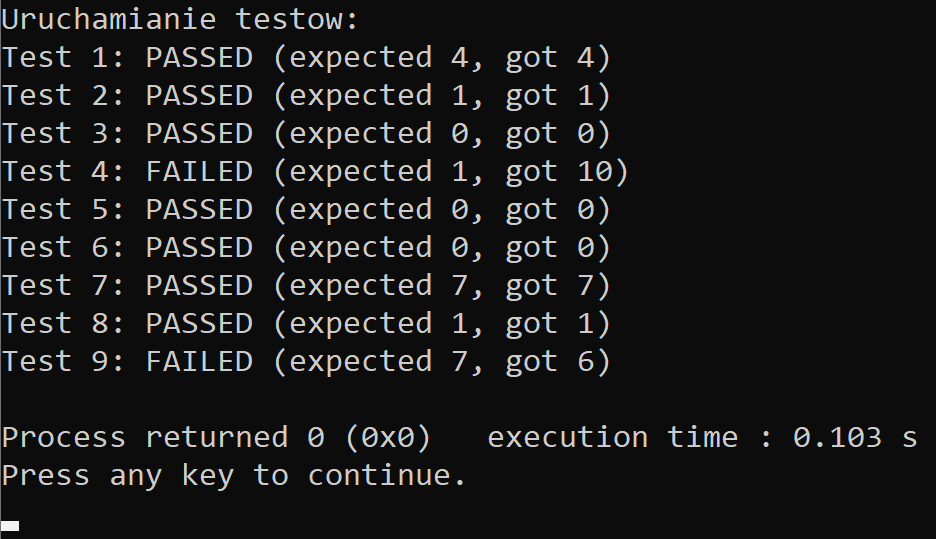
\includegraphics[width=1\textwidth]{Test1.png}
    \caption{Pierwsze testy drugiego programu (funkcja \texttt{RunTests}).}
    \label{fig:Test1}
\end{figure}

Na widocznym zrzucie ekranu z okna konsoli można zaobserwować wyniki przeprowadzonych testów, które zostały wcześniej utworzone w kodzie. Dla utworzonych tablic sprawdzamy, czy obliczona wartość malejących podciągów jest równa wartości oczekiwanej, czyli obliczonej przez nas liczbie. Jeśli te wartości się pokryją to program wypisze na ekranie \texttt{PASSED} wraz z oczekiwaną i otrzymaną wartością, ale jeśli obliczy wartość inną niż oczekiwaliśmy, to wyświetli \texttt{FAILED} wraz z obliczoną i oczekiwaną wartością (na potrzeby pokazania tej funkcji we wcześniejszej deklaracji testów dwie oczekiwane wartości zostały ustawione na niepoprawne).
\rule{0cm}{0.1cm} % przerwa miedzy tekstem
\begin{figure}[H]
    \centering
    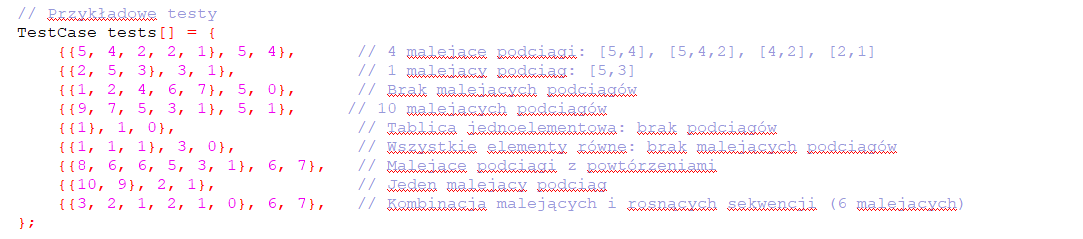
\includegraphics[width=1\textwidth]{Test2.png}
    \caption{Przypomnienie deklaracji przykładowych testów w funkcji \texttt{RunTests}.}
    \label{fig:Test2}
\end{figure}

\rule{0cm}{0.1cm} % przerwa miedzy tekstem

Widać, że tam gdzie w komentarzu wypisana jest informacja o 10 malejących podciągach, w deklaracji oczekiwanej wartości jest wpisane 1, stąd pojawia się komunikat \texttt{FAILED} w oknie konsoli (analogicznie w przypadku testu numer 9).

\newpage

\section{Testowanie}

Na poniższym wykresie przedstawię porównanie liczby operacji w dwóch przypadkach:
\begin{enumerate}
\item{Wykonanie zadanie w pełni tak, jak jest to oczekiwane (wypisanie wszystkich podciągów malejących oraz ich liczby).}
\item{Wykonanie zadania częściowo przy użyciu funkcji \texttt{CountDecreasingSubarrays} (wypisanie tylko liczby malejących podciągów.}

(\textbf{UWAGA:} Liczba operacji zostanie zliczona poprzez dodanie zmiennej pomocniczej, która zwiększy się o 1 przy każdym wykonaniu się danego fragmentu kodu).

\begin{figure}[H]
    \centering
    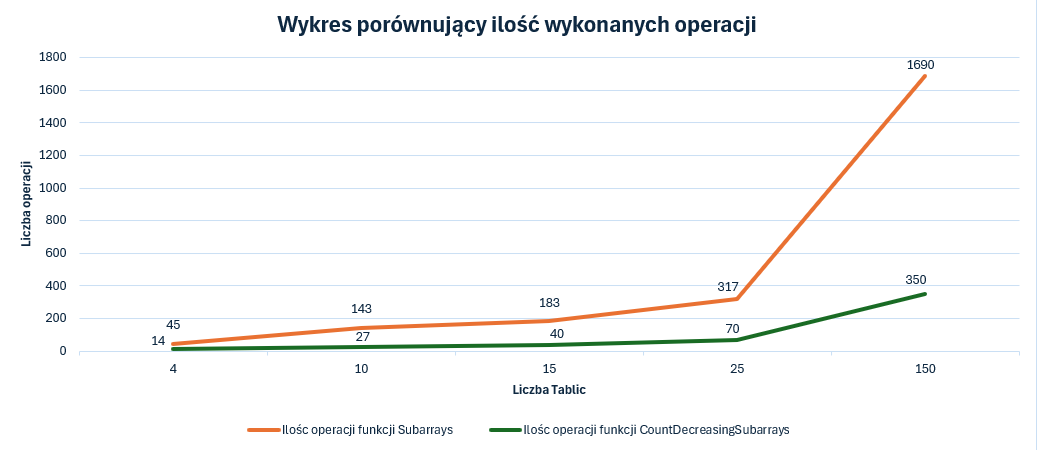
\includegraphics[width=1\textwidth]{Wykres1.png}
    \caption{Wykres porównujący ilość wykonanych operacji w zależności od liczby tablic.}
    \label{fig:Wykres1}
\end{figure}

Można zaobserwować, że funkcja \texttt{CountDecreasingSubarrays} odpowiedzialna tylko za obliczenie liczby podciągów malejących wykonała mniej operacji aniżeli funkcja \texttt{Subarrays}.

\end{enumerate}

\rule{0cm}{0.5cm} % przerwa miedzy tekstem

\section{Podsumowanie i wnioski}

Podczas realizacji tego projektu zobaczyliśmy jak można rozwiązać problem wyszukiwania malejących podciągów w tablicy oraz porównaliśmy dwa sposoby rozwiązywania jednego polecenia. Mimo tego, że złożoność obliczeniowa wyszła O(n\textsuperscript{3}) to niestety bardzo trudno byłoby osiągnąć mniejszą złożoność, zakładając że chcemy, aby program spełniał wszystkie wymogi. Z tego też powodu program może się nie nadawać do pracy z dużą ilością tablic. Z naszych testów także wynika, że jeśli zależy nam tylko na uzyskaniu odpowiedzi na pytanie "Ile jest malejących podciągów?", to warto jest zastosować funkcje, które są bardziej wydajne i mniej złożone. 

\end{document}
